\begin{frame}\frametitle{Performing Localisation in Real Missions}
\begin{block}{Spiral surfacing trajectory}
\begin{columns}
\column{.7\textwidth}
Spiral trajectory and surfacing action was taken with Nessie starting from the depth of around 12 m (Fig. ~\ref{fig:spiral}). %Trajectory seems to be smoother and less prone to drift . %Standard deviation of north and east measurement noise can be set 
\column{.28\textwidth}
\centering
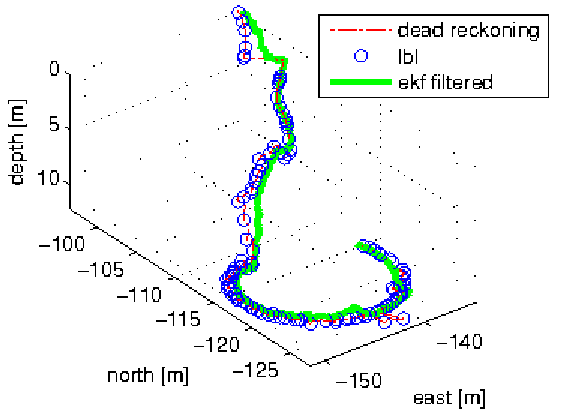
\includegraphics[width=0.7\linewidth]{fig/spiral3d.pdf}
\end{columns}
\end{block} 
\centering 
\begin{figure}
\vspace{-15pt}
\caption{Spiral trajectory localisation}
\vspace{-15pt}
\subfigure[{\scriptsize N/E localisation}]{\label{fig:ne2d}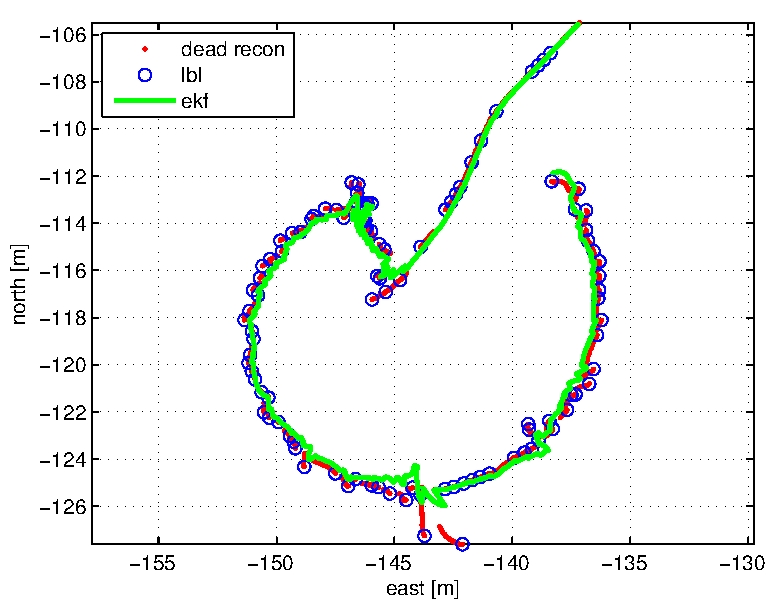
\includegraphics[width=0.45\linewidth]{fig/spiral2d.pdf}}
\subfigure[{\scriptsize depth filtering}]{\label{fig:depth}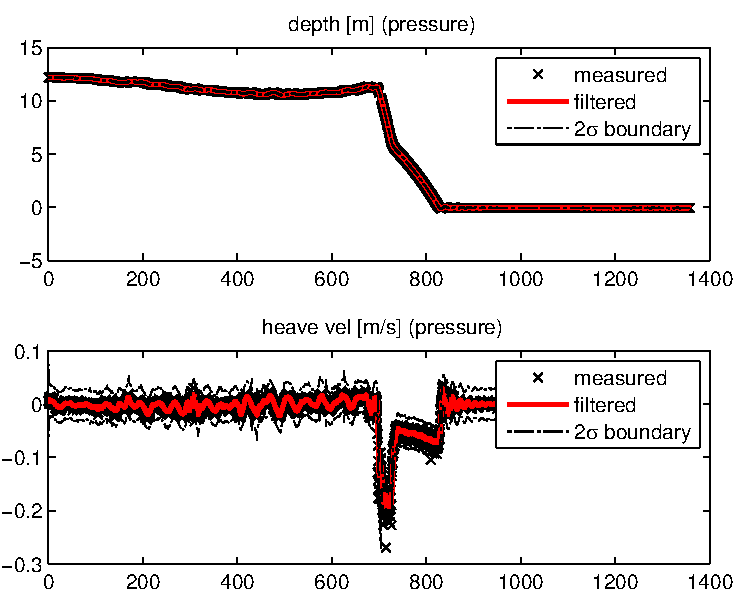
\includegraphics[width=0.45\linewidth]{fig/spiral-depth.pdf}} \\
\label{fig:spiral}
\end{figure}
%\begin{columns}[t]
%\column{.5\textwidth}
%\column{.2\textwidth}
\end{frame}